% ============================================================================
%  SSEE — Cosmological Cover / Title page
%  Real Hubble galaxy photograph (public domain, NASA/ESA) as background,
%  with SSEE's own equations as a faint scholarly texture, and elegant
%  typography.  University-monograph look + the beauty of the real universe.
%  Background image: cover_galaxy.jpg  (M51 Whirlpool — swap for
%  cover_galaxy_ngc1300.jpg to use the barred spiral).
%  Compile:  pdflatex SSEE_Cover.tex   (twice)
% ============================================================================
\documentclass[11pt]{article}
\usepackage[paperwidth=210mm,paperheight=297mm,margin=0pt]{geometry}
\usepackage[T1]{fontenc}
\usepackage[utf8]{inputenc}
\usepackage{amsmath}
\usepackage{graphicx}
\usepackage{tikz}
\usetikzlibrary{calc,fadings}
\usepackage{xcolor}
\usepackage{microtype}
\pagestyle{empty}

\definecolor{spaceblack}{HTML}{03040A}
\definecolor{ssgold}{HTML}{D9B45A}
\definecolor{ssgoldlt}{HTML}{F0D28A}
\definecolor{cream}{HTML}{F5F1E6}
\definecolor{slate}{HTML}{B9C1DC}

% vertical alpha gradients for legibility scrims
\tikzfading[name=downfade, top color=transparent!100, bottom color=transparent!0]
\tikzfading[name=upfade,   top color=transparent!14, bottom color=transparent!100]

\begin{document}
\begin{tikzpicture}[remember picture, overlay]

  % --- base + full-bleed galaxy photograph ------------------------------
  \fill[spaceblack] (current page.south west) rectangle (current page.north east);
  \begin{scope}
    \clip (current page.south west) rectangle (current page.north east);
    \node at (current page.center)
      {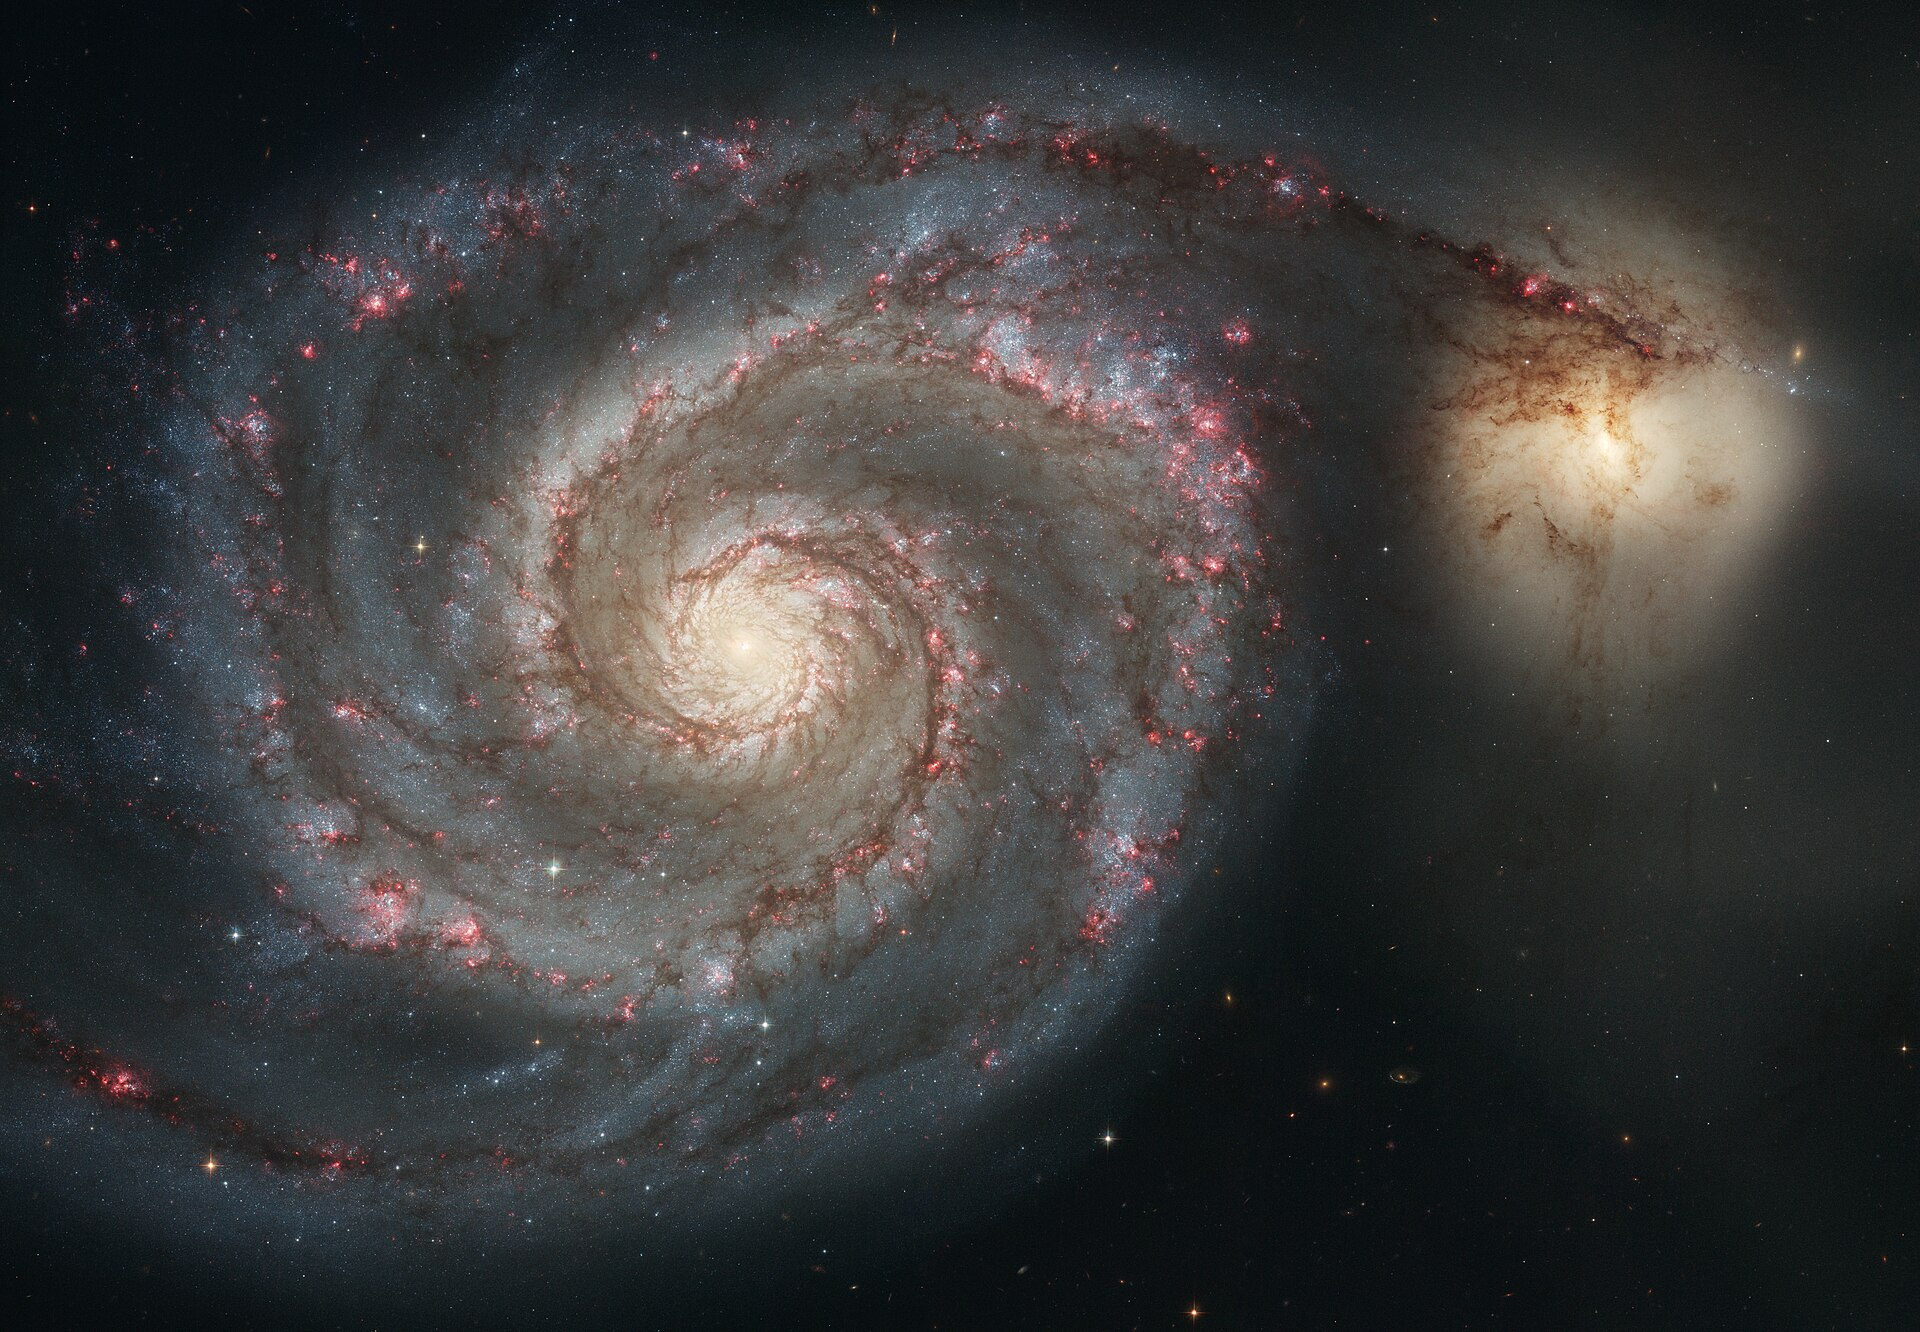
\includegraphics[height=1.02\paperheight]{cover_galaxy.jpg}};

    % --- faint SSEE equations: scholarly texture over the dark field ----
    \foreach \eq/\px/\py/\rot/\op in {%
      {$\Omega=\varphi+\pi$}/-6.6/9.2/-8/0.13,
      {$w_0=-T_r/M_v=-0.840$}/4.9/12.3/6/0.11,
      {$n_s=1-\varphi^{-7}$}/-7.2/-3.1/9/0.12,
      {$w_a=-P_{\rm sc}/K_v=-0.670$}/5.6/-8.7/-7/0.11,
      {$f_{\rm screen}=\dfrac{\pi-\varphi}{(\varphi+\pi)^2}$}/-6.1/-10.6/8/0.10,
      {$\Omega_m=\omega_m/h^2$}/6.6/2.2/-6/0.11,
      {$H_0/(\mathrm{km\,s^{-1}Mpc^{-1}})=3(\varphi+\pi)^2$}/0/-12.4/0/0.10,
      {$k_{\rm fs}=0.754\,h\,\mathrm{Mpc}^{-1}$}/-5.7/5.0/7/0.10%
    }{
      \node[text=cream, opacity=\op, font=\small, rotate=\rot]
            at ($(current page.center)+(\px,\py)$) {\eq};
    }

    % --- legibility scrims (bottom drawn thrice for a solid title bed) --
    \fill[spaceblack, path fading=downfade]
        (current page.south west) rectangle ($(current page.south east)+(0,18cm)$);
    \fill[spaceblack, path fading=downfade]
        (current page.south west) rectangle ($(current page.south east)+(0,13cm)$);
    \fill[spaceblack, path fading=downfade]
        (current page.south west) rectangle ($(current page.south east)+(0,9cm)$);
    \fill[spaceblack, path fading=upfade, opacity=0.92]
        (current page.north west) rectangle ($(current page.south east)+(0,24.2cm)$);
  \end{scope}

  % --- thin gold frame --------------------------------------------------
  \draw[ssgold, line width=0.7pt, opacity=0.85]
     ($(current page.south west)+(11mm,11mm)$) rectangle
     ($(current page.north east)+(-11mm,-11mm)$);

  % --- kicker: reads instantly as cosmology -----------------------------
  \node[anchor=north, text=ssgoldlt, font=\sffamily\bfseries, yshift=-22mm]
        at (current page.north) {\textls[440]{\large C O S M O L O G Y}};
  \node[anchor=north, text=slate, font=\sffamily\footnotesize, yshift=-31mm]
        at (current page.north) {\textls[340]{THE DARK-ENERGY UNIVERSE}};

  % --- title (lower third, over the scrim) ------------------------------
  \node[text=cream, font=\fontsize{43}{49}\selectfont\bfseries, align=center,
        yshift=78mm] at (current page.south)
        {Structural\\[1pt] Self-Energy\\[1pt] Expansion};

  \draw[ssgold, line width=0.8pt, opacity=0.9]
      ($(current page.south)+(-4.7cm,50mm)$) -- ($(current page.south)+(4.7cm,50mm)$);

  \node[text=ssgoldlt, font=\itshape\large, align=center, yshift=42.5mm]
        at (current page.south)
        {A Minimal-Parameter Dark-Energy Framework};
  \node[text=slate, font=\itshape\normalsize, align=center, yshift=37mm]
        at (current page.south)
        {anchored in the golden ratio $\varphi$ and $\pi$};

  % --- author block (bottom) -------------------------------------------
  \node[anchor=south, text=cream, font=\sffamily\Large\bfseries, yshift=23mm]
        at (current page.south) {Mike Edison Almeida Vallejo};
  \node[anchor=south, text=slate, font=\sffamily\small, yshift=17mm]
        at (current page.south) {\textls[220]{INDEPENDENT RESEARCHER}};
  \node[anchor=south, text=slate, font=\sffamily\scriptsize, yshift=12mm]
        at (current page.south) {ORCID 0009-0008-2195-7836 \quad$\cdot$\quad 2026};

  % --- image credit (licensing; discreet, in the bottom margin) ---------
  \node[anchor=south, text=slate, opacity=0.65, font=\fontsize{5.4}{6}\selectfont, yshift=5mm]
        at (current page.south)
        {Cover image: NASA, ESA \& the Hubble Heritage Team (STScI/AURA)\,---\,Messier\,51 (public domain)};

\end{tikzpicture}
\end{document}
